\section{\sys in Reliable Networks}
\label{sec:design-reliable}

%\begin{figure}[t]
%\centering
%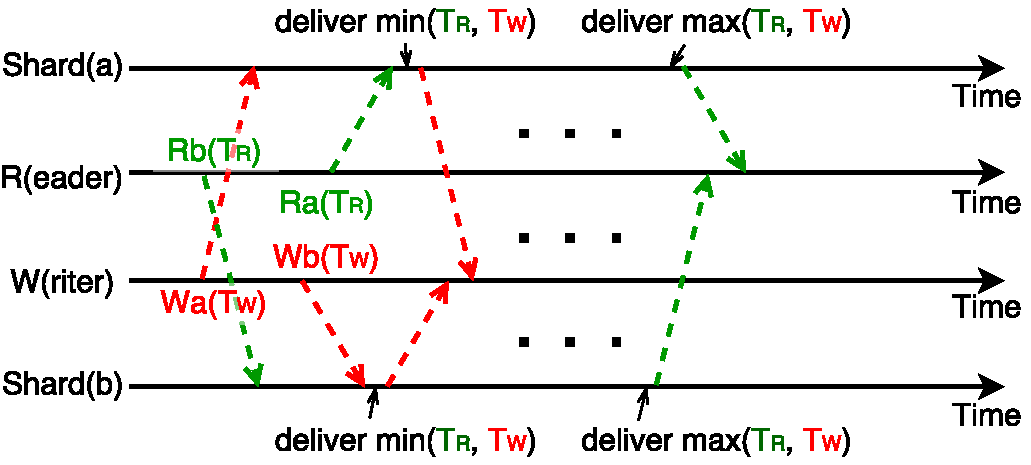
\includegraphics[width=0.48\textwidth]{images/derive_barriers.pdf}
%\caption{Deriving barriers with senders $R, W$ and receivers Shard($a$), Shard($b$).}
%\label{fig:barrier}
%\vspace{-1em}
%\end{figure}

In this section, we assume that the network is reliable. There is no host, link or switch failure. No packet is lost due to congestion or corruption. We make such strong assumptions to help reader understand the key ideas of \sys. We will present the design in lossy and failure-prone networks in Sec.\ref{sec:design-unreliable}.


%\textbf{Scalability}.
%If there are $N$ senders and $N$ receivers, the complexity of communication is $O(N^2)$.
%Sec.\ref{sec:ideal} leverages network switches to merge beacons hierarchically and reduce the beacon message complexity to $O(N)$.

%\textbf{Liveness}.
%If either $R$ or $W$ stops sending messages, shard($a$) can not deliver messages with timestamps higher than $\min(T_R,T_W)$, causing a livelock.
%To ensure liveness, each network link sends \textit{beacon} messages periodically (Sec.\ref{sec:beacon}).

%\textbf{Reordering delay}.
%To minimize \textit{reordering delay}, which is the delay between receiving and delivering a message, Sec.\ref{sec:sync} synchronizes clocks at senders.

%\textbf{Packet loss}.
%If a packet is lost, the receivers will observe an incomplete ordering of events.
%Simple retransmission with same timestamp violates the monotonic property of timestamps.
%The detection and recovery of packet losses are discussed in Sec.\ref{sec:lossy}.

%\textbf{Fault tolerance}.
%Sec.\ref{sec:failure} discusses how to add end hosts, switches and links on the fly, with minimal impact on system performance, and how to merge two existing \sys systems.

%\textbf{Inter-DC topology}.
%Sec.\ref{sec:inter-dc} extends the design to inter-DC topology where routing paths are not loop-free.


%\subsection{Hierarchical Merge of Barriers}
\subsection{Message and Barrier Timestamp}
\label{sec:ideal}

\begin{figure}[t]
\centering
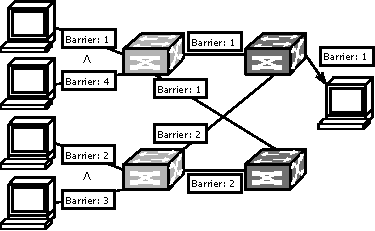
\includegraphics[width=0.4\textwidth]{images/hierarchical_merge.pdf}
\caption{Hierarchical aggregation of barrier timestamp.} %\RED{Change logos smaller. Use computer logo instead of this logo. Make the network links vertical (orthogonal to horizontal). MODIFIED, NEED REVIEW}
\label{fig:hierarchical_merge}
\vspace{-0.9em}
\end{figure}

\parab{Message timestamp.}\sys assigns a non-decreasing timestamp for each message. A set of messages with an identical timestamp forms a scattering, while different scattering are assigned different timestamps. %Each sender assigns monotonically increasing message timestamps, \textit{e.g.}, synchronized physical time, to different scatterings. 
Message timestamp determines the processing order at receiver. To achieve ordered message scattering, the receivers should process arrival messages in ascending order of their timestamps (ties are broken through host ID). Here we use ``process'' and ``delivery'' interchangeably. 

\parab{Barrier timestamp.} When a receiver wants to process a message with timestamp $t$, it must be sure that it has received and processed all the messages whose timestamps are smaller than $t$. Since messages can be received out of order, this is nontrivial. To this end, we introduce the concept of \emph{barrier timestamp}. A barrier timestamp is associated with either a link or a node (i.e. a switch or an end host) in the routing graph. The barrier timestamp is the lower bound of message timestamps of all \emph{future arrival messages} from the link, or at the node. Each receiver can maintain its own barrier timestamp and process the messages whose timestamps are smaller than the barrier timestamp.

Due to non-decreasing timestamp assignment, in a FIFO network (such as by using TCP transport), a receiver can easily figure out the barrier if it has received messages from all senders: the barrier is the minimum timestamp of latest messages from each sender. Therefore, a naive solution would be for every sender to send periodic beacons to every receiver so that the receivers can figure out the barrier and process messages. Unfortunately, such a solution requires quadratic beacons.

%We use a simple example to show how to derive the barrier timestamp. In Figure~\ref{fig:barrier}, there are two senders $R$, $W$ and two receivers shard($a$) and shard($b$). $R$ issues a scattering with message $R_a$ and $R_b$ to read data from shard($a$) and shard($b$), respectively. The message timestamp is $T_R$. In the meanwhile, $W$ issues a scattering with message $W_a$ and $W_b$ to write data to shard($a$) and shard($b$), respectively. The message timestamp is $T_W$. When shard($a$) receives both $R_a$ and $W_a$, due to monotonic message timestamp assignment, shard($a$) knows that it will not receive messages with timestamp $T \le T_R$ from $R$ or $T \le T_W$ from $W$. Further, shard($a$) will not receive messages with timestamp $T \le \min(T_R, T_W)$ from either $R$ or $W$. Hence, shard($a$) derives a barrier timestamp $\min(T_R, T_W)$ and it can process all messages with timestamp $T \le \min(T_R, T_W)$.



%\sys leverages the \emph{barrier timestamp} to provide order information. Before going to the mechanims, we illustrate the barrier timestamp with a simple example.

%In Figure~\ref{fig:barrier}, there are two senders $R$, $W$ and two receivers shard($a$) and shard($b$). $R$ issues a scattering with message $R_a$ and $R_b$ to read data from shard($a$) and shard($b$), respectively. In the meanwhile, $W$ issues a scattering with message $W_a$ and $W_b$ to write data to shard($a$) and shard($b$), respectively. Each sender assigns an identical timestamp for all the messages in a scattering, namely $T_R$ and $T_W$. Each sender assigns monotonically increasing timestamps to different scatterings. Message timestamp determines the processing order at receiver. When shard($a$) receives both $R_a$ and $W_a$, due to monotonic timestamp assignment, shard($a$) knows that it will not receive messages with timestamp $T \le T_R$ from $R$ or $T \le T_W$ from $W$. Further, shard($a$) will not receive messages with timestamp $T \le \min(T_R, T_W)$ from either $R$ or $W$. Hence, shard($a$) can process all messages with timestamp $T \le \min(T_R, T_W)$. In this example, each receiver actually derives a \textit{barrier timestamp}, \textit{e.g.}, $\min(T_R, T_W)$, which is the minimum message timestamp of all possible senders.

\parab{Hierahical barrier timestamp aggregation.} The naive solution discussed does not scale in production data centers. \sys leverages programmable switches to \emph{aggregate} the barrier timestamp information. Given the limited switch buffer resource, \sys does not reorder messages in the network. Instead, \sys forwards messages in the network as usual, but reorders and processes them at the receiver side based on the barrier timestamp information provided by the switch.

In \sys, we attach two timestamp fields to each message packet. The first is \textit{message timestamp} field, which is set by the sender and will not be modified. The second field is \textit{barrier timestamp}, which is initialized by the sender but will be modified by switches along the network path. The property of the barrier timestamp field is:

\emph{When a switch or a host receives a packet with barrier timestamp $B$ from a network link $L$, it indicates that the message timestamp and barrier timestamp of future arrival packets from link $L$ will be larger than $B$.}

To derive barriers, the sender initializes both fields of all packets in a message\footnote{A large message may consist of multiple packets.} with the non-decreasing message timestamp. The switch maintains a register $R_i$ for each input link $i \in \mathcal{I}$, where $\mathcal{I}$ is the set of all input links. After forwarding a packet with barrier timestamp $B$ from input link $i$ to output link $o$, the switch performs two updates. First, it updates register $R_i := B$. Second, it modifies the barrier timestamp of the packet to $B_{new}$ as follows:

%\RED{$i$ never appeared before, while $I$ did. $\exists$ is redundant}
\begin{equation}\label{equ:derive_barriers}
%\RED{
B_{new}:=\min\{R_i| i\in \mathcal{I}_o\}
%}
\end{equation}
%B := \min \{ R_i | \exists i \rightarrow E, i \in \mathcal{I} \}
Where 
\begin{equation}\label{equ:derive_barriers1}
\mathcal{I}_o =\{i| i\rightarrow o, i \in \mathcal{I} \}
\end{equation}

Here $\rightarrow$ means \textit{can be forwarded to}. In the regular topologies of data centers, the set of all possible input links $\mathcal{I}_o$ is predetermined at route configuration time. Using (\ref{equ:derive_barriers}) and (\ref{equ:derive_barriers1}), each switch independently derives the barrier timestamp based on all possible input links. As shown in Figure~\ref{fig:hierarchical_merge}, barrier timestamps are aggregated hierarchically through layers of switches, and finally the receiver gets the barrier of all reachable hosts and links in the network. In Appendix~\ref{appx:hierarchical_merge}, we prove that this algorithm maintains the property of barrier timestamps, given the FIFO property of each network link and switch.

When the receiver receives a packet with barrier timestamp $B$, it first buffers the packet in a priority queue that sorts packets based on the message timestamp. The receiver knows that the message timestamp of all future arrival packets will be larger than $B$. Hence, it delivers all buffered packets with the message timestamp below $B$ to the application for processing.




%One liveness requirement of the system is \textit{Loop-Free Routing}(Sec.\ref{sec:assumptions}).
%{The liveness of the system is guaranteed if there are no \textit{routing loops} in the network (Sec.\ref{sec:assumptions}).}
%If there is a routing loop of links $L_1, \ldots , L_n$, then the barrier timestamps $B_{L_2} \leq B_{L_1}, \ldots, B_{L_n} \leq B_{L_{n-1}}, B_{L_1} \leq B_{L_n}$.
%So we can't increase the barrier timestamp because a packet may be forwarded in this routing loop indefinitely.
%{, so the barrier timestamps cannot increase.
%This result is evident because a packet may be forwarded in this routing loop indefinitely, therefore we cannot increase the lower bound of in-flight message timestamps.}
%When the routing loop is removed, barrier timestamps will start increasing again.

%Although the design above works on a reconfigurable switch, many fixed function switching chips are not capable of storing states $R_i$ and calculating the minimum among $R_i$.
%We offload the control plane to the CPU on switches, by using beacon packets as \textit{slacked barriers} of data packets.
%This will be discussed in Sec.\ref{sec:commodity}.

\subsection{Beacons on Idle Links}
\label{sec:beacon}

As shown before, at each hop, the per-packet barrier timestamp is updated to the minimum barrier timestamp value of all possible input links.
As a result, an idle link can keep the per-packet barrier timestamp unchanged, thus throttling the whole system.
To avoid idle links, we send \textit{beacons} periodically on every link.


%Therefore, the liveness of \sys requires information from every network link. The receiver cannot distinguish between an idle link and a link with excessive delay.
% should be "between A and B" or "either A or B", see here https://english.stackexchange.com/questions/138239/between-with-and-or-or

\parab{What is a beacon?}Unlike the message packet, the beacon packet only carries the barrier timestamp field and has no payload data, thus minimizing network overhead. 

\parab{How to send beacons?}A simple approach is to let all the senders to send beacons to all the receivers. This approach has two limitations. First, it causes high bandwidth overhead as a link may be covered by multiple beacons. Second, it cannot guarantee to cover every link.

Instead, we send beacon packets on a per-idle-link basis.
The beacon packet can be sent by both the hosts and the switches,
but the destination must be its one-hop neighbors. For a beacon generated by the host, the barrier timestamp field is initialized in the same way as the regular message packet. For a beacon generated by the switch, the barrier timestamp field is initialized according to Equation \ref{equ:derive_barriers} and \ref{equ:derive_barriers1}.

\parab{When to send beacons?}
We introduce a beacon interval $T_{beacon}$. When a host or a switch output link does not observe any message packet for $T_{beacon}$ time, it generates a beacon packet. We should choose a suitable $T_{beacon}$ to balance the trade off between overhead and reordering delay. We set $T_{beacon}$ to 10us by default in the evaluation.

%The choice of $T_{beacon}$ is a trade-off between overhead and reordering delay.
%The reordering delay may increase by at most $T_{beacon}$ because the receiver of an idle link can only increase its barrier timestamp every time it receives a beacon.

%There are two ways: (1) let the sender send a signal packet to shutdown the link temporarily; (2) ensure the link is always busy by sending periodic \textit{beacons}.

%The first solution requires the sender to rejoin the receiver when it has another packet to send, which requires at least a single-hop RTT to re-sync the timestamps (Sec.\ref{sec:failure}). Therefore, this solution is applicable when the sender knows it would not send any packet during a relatively long period, \textit{e.g.}, when the application closes.

%Beacons not only introduce network and CPU overhead, but also affects reordering delay.
%The receiver of an idle link can only increase its barrier timestamp every time it receives a beacon.
%We further synchronize beacons at different network links, so that reordering delay overhead is the beacon interval regardless of number of hops in network path.
%To this end, we introduce two beacon intervals $B_{min}$ and $B_{max}$.
%A switch broadcasts beacons as soon as it receives a beacon and have not sent beacons for at least $B_{min}$ time.
%A switch also broadcasts beacons when it has not received a beacon for $B_{max}$ time.
%$B_{min}$ is set to the estimated maximum path delay variance, while $B_{max}$ is the desired beacon interval.
%Choosing $B_{max}$ is a trade-off between the network/CPU overhead and reordering delay.


\iffalse
%Remove the algorithm because it does not contain much information and takes too much space.
\setlength{\textfloatsep}{1em}
\begin{algorithm}[t]
 \DontPrintSemicolon
 \textbf{Parameters:} beacon intervals $min$, $max$\;
 \textbf{States:} Ingress port barrier timestamp $R_i, i \in \mathcal{I}$\;
   \qquad Egress port barrier timestamp $B_e, e \in \mathcal{E}$\;
   \qquad Last sent barrier time last$_e, e \in \mathcal{E}$\;
   \qquad Local physical clock, fetched via \textit{time()}\;
   \qquad timer$_e, e \in \mathcal{E}$ that fires after a given interval\;
 \SetKwProg{Fn}{Function}{ begin}{end}
 \SetKwFunction{SendBeacon}{SendBeacon}
 \Fn{\SendBeacon{\textnormal{barrier} $B_E$, \textnormal{output link} $E$}}{
    Send beacon packet $B_E$ to $E$\;
    last$_E \leftarrow$ time()\;
    reset timer$_E$ to fire after $max$\;
 }
 \SetKwFunction{UpdateEgressPortTS}{UpdateEgressPortTS}
 \Fn{\UpdateEgressPortTS{\textnormal{output link} $E$}}{
    $B_E \leftarrow \min \{ R_i | i \rightarrow E, i \in \mathcal{I} \}$\;
    \eIf{last$_E + min \leq$ time()}{
      SendBeacon ($B_E$, $E$)\;
    }{
      reset timer$_E$ to fire after last$_E + min - $time()\;
    }
 }
 \textbf{Event processing:}\\
 \If{receive a beacon or data packet $P$}{
  read barrier timestamp $b$ from packet $P$\;
  $R_I \leftarrow b$, where $I$ is the input link of $P$\;
  \If{$P$ is a data packet}{
  	determine output link $E$ of $P$ by routing\;
    UpdateEgressPortTS ($E$)\;
    modify barrier timestamp in $P$ to $B_E$\;
  }
  \ElseIf{$P$ is a beacon packet}{
  	\ForEach{$e \in \{ e \in \mathcal{E} | I \rightarrow e \}$}{
    	UpdateEgressPortTS ($e$)\;
    }
  }
 }
 \ElseIf{timer$_E, E \in \mathcal{E}$ fires}{
    SendBeacon ($B_E$, $E$)\;
 }
 \caption{Timestamp processing with beacons.}
 \label{alg:beacon}
\end{algorithm}
\fi

%In order to detect failures, each switch has a timeout timer per input link. If no beacon or data packet is received for three max beacon intervals, the input link is considered to be dead and removed from the input link list. When the failed link, host or switch recovers, it needs to rejoin (Sec.\ref{sec:incremental}).

\subsection{Minimax Clock Synchronization}
\label{sec:sync}

%\RED{\sout{People perceive two events as simultaneous when observing their effects at the same time.}}
%Due to different propagation delays from the origin of events to the observers, simultaneity of events is relative to observers.
%From an end-host receiver's perspective, two events should be simultaneous if the messages originated from the events arrive at the receiver simultaneously.
%In a distributed system, events are timestamped and their effects propagate in the form of packets.
%On one hand, we hope to timestamp the events so that if two packets originated from two distant events arrive at a receiver simultaneously, these two events should have a same timestamp.
%On the other hand, unlike our physical universe, a distributed system is easier to reason if the ordering of events is globally consistent, \textit{i.e.}, all receivers agree on the timestamps of events.

\parab{Timestamp Assignment.}An immediate question is how to assign message timestamps. Given recent efforts on accurate clock synchronization~\cite{correll2005design,corbett2013spanner,lee2016globally,geng2018exploiting}, a straightforward solution is to use \emph{physical} time. When a host scatters a group of messages, it uses current physical time to initialize message timestamp and barrier timestamp fields of all packets.

However, this approach does not take into account the delay variance of different network paths. Delay variance is caused by the variance of processing delays in OS kernel, queuing delays at the switch and different number of network hops. The delay variance causes straggler problem. Consider two independent messages being sent from two senders to the same receiver at the same physical time. They might arrive at different times due to different network delays. As a result, the earlier message must wait for the later one to be processed together, which increases reordering delay.

%The next challenge is how to assign timestamps to messages.
%Clock synchronization in data centers becomes increasingly accurate leveraging NIC timestamps~\cite{correll2005design}, GPS~\cite{corbett2013spanner}, PHY~\cite{lee2016globally} and network effects~\cite{geng2018exploiting}.
%However, delay variance of network paths makes physical time a suboptimal choice for timestamps.
%Different OS network stacks have more than 100~$\mu$s of processing delay differences, and it may increase to milliseconds under heavy load.
%Links with different speeds or congestion also lead to delay variations.
%For example, two messages are transmitted from two senders to the same receiver at the same physical time.
%However, they arrive at different times due to different network delays.
%As a result, the earlier one must wait for the later one to be processed together, which increases reordering delay.

\parab{Logical time.}In \sys, we use \emph{logical time} as the message timestamp. Loosely speaking, logical time is essentially the estimated message arrival time, \emph{i.e.}, receiver's clock time plus one way delay from the sender to the receiver.
Logical time roughly increases at the same rate as the clock time, therefore, in practice, we represent logical time as local clock time plus an offset, and track and adjust the offset instead.

\parab{Logical time synchronization.}We observe that clock drift is small (relative error less than $10^{-5}$~\cite{corbett2013spanner,geng2018exploiting}), and consider physical clocks precise enough to measure short intervals. We begin with the simplest case with a single sender $S$ with its local clock $T_s$ and a single receiver $R$ with local clock $T_r$. We want to find an adjustment offset $O_s$ such that if $T = T_s + O_s$ is used as the message timestamp at $S$, when the message arrives at $R$, $R$'s local time $T_r$ is equal to $T$. In the network, measuring the one way delay directly from $S$ to $R$ or from $R$ to $S$ is hard, but the round-trip time between two nodes is easy to measure, and we assume it is known as $RTT_{sr}$.

We can use the following protocol to figure out $O_s$. Let $R$ send a clock sync message to $S$ at time $T_{r0}$ and attach the value of $T_{r0}$ in the message. $S$ receives it at $T_{s0}$ according to its local clock. Imagine that $S$ immediately replies the message to $R$ with timestamp $T = T_{s0} + O_s$, then $R$ will receive the reply at $T' = T_{r0} + RTT_{sr}$. To make $T$ equals $T'$, we only need to adjust $O_s$ to be $T_{r0} + RTT_{sr} - T_{s0}$. Since $S$ knows $T_{s0}$ when it receives the message, and can obtain $T_{r0}$ from the message, it can adjust $O_s$ as soon as it receives the clock sync message.



%We begin with a simplistic case with multiple senders $S_i \in \mathcal{S}$ and one receiver $R$.
%Assume the one-way network delays are forward delays $f_i$ for $S_i \rightarrow R$ and backward delays $b_i$ for $R \rightarrow S_i$.
%Note that we can measure the round-trip time ($RTT_i = f_i + b_i$) between two nodes, but one-way delay is hard to measure.
%
%To minimize reordering delay, we want messages with similar \textit{message timestamps} arrive at the receiver around the same time.
%\REDBLU{
%	If R broadcasts a clock synchronization message to set logical time to 0 at physical time 0, $S_i$ will receive it at $r_i$.
%	Then $S_i$ compensates $RTT_i$ to the received timestamp and sets its logical time to $d_i+r_i$.
%	If each $S_i$ immediately reply to $R$ with the new logical time, $R$ will receive message with logical time $d_i+r_i$ at physical time $d_i+r_i$, which theoretically means zero reordering delay.
%}
%{
%Consequently, the logical clock at $S_i$ should have an offset $d_i$ to the physical time.
%If $R$ broadcasts a clock synchronization message at physical time 0, $S_i$ will receive it at $r_i$.
%Then $S_i$ compensates a round-trip time $RTT_i$ to the received timestamp and sets its clock to $0 + d_i + r_i$ at physical time $r_i$, which has offset $d_i$ to physical time.
%Our goal is achieved.
%}

%\begin{algorithm}[t]
% \DontPrintSemicolon
% \textbf{States:} Clock adjustment offset $off$\;
% \qquad Last assigned timestamp $T_{last}$\;
% \qquad Local physical clock, fetched via $time()$\;
% \textbf{Event processing:}\;
% \If{received sync timestamp $T_{sync}$}{
% 	$off \leftarrow T_{sync} - time()$\;
% }
% \ElseIf{a total-ordered event occurs}{
%    TS $\leftarrow \max (T_{last} + 1, time() + off)$\;
%    $T_{last} \leftarrow$ TS\;
% }
% \caption{Clock adjustment and timestamp assignment on each end host.\RED{To be revised}}
% \label{alg:clock}
%\end{algorithm}

\begin{algorithm}[t]
\DontPrintSemicolon
\textbf{Variables:}\;
Logical time adjustment offset $S$: $O_{s}$\;
Local physical clock time: $time()$\;
Round-trip time between $S$ and $R$: $RTT_{sr}$\;
Message timestamp: $T$\;
Last assigned message timestamp: $T_{last}$ \;
\;
\textbf{Event processing:}\;
\If{receive a clock sync message from host $R$ with $T_{r0}$}{
	$O_{s} \leftarrow T_{r0} + RTT_{sr}  - time()$\;	
}
\ElseIf{scatter a group of messages}{
	$T \leftarrow \max(T_{last} + 1, time() + O_{s})$\;
    $T_{last} \leftarrow T$
}
\caption{Logical time synchronization and timestamp assignment at the host $S$}
\label{alg:clock}
\end{algorithm}

%\parab{Adjust logical time}
Because message timestamps can not decrease, when the new offset $O_s^{new}$ is smaller than $O_s^{old}$, the system has to ``stall'' the logical clock rather than decrease it.
During stall, the offset $O_s$ is adjusted so that the logical clock increases by 1 per scattering until it reaches the target offset $O_s^{new}$. Algorithm~\ref{alg:clock} shows the procedure. This algorithm can be trivially extended to the case where there are multiple senders $S_i \in \mathcal{S}$, making all the senders be synchronized to the receiver's local clock time.

Now we extend to multiple receivers $R_i \in \mathcal{R}$.
%In a data center, each sender is also a receiver, but we denote the send and receive roles separately for clarity.
Assume the one-way forward delay is $f_{ij}$ for $S_i \rightarrow R_j$ and backward delay is $b_{ij}$ for $R_j \rightarrow S_i$, and we can measure $RTT_{ij} = f_{ij} + b_{ij}$.
If we want to follow the approach above for each receiver, we need to synchronize the clocks of receivers first.
In this regard, we add a \textit{forward pass} in which every sender $S_i$ sends clock sync messages to every receiver $R_j$ to synchronize the clock of $R_j$, then run the \textit{backward pass} like above from $R_j$ to $S_i$.
In both passes, each node can calculate potentially different offset adjustments from multiple peers, so we need two aggregation functions to resolve conflicts, namely \texttt{FwdFunc} and \texttt{BackFunc}.
Assume the sender logical clocks are $T_k, k \in \mathcal{S}$ initially, the new logical clocks $T'_k$ after two passes should be:
$T'_k  = \texttt{BackFunc}_k \{ \texttt{FwdFunc}_j \{ T_i | i \in \mathcal{S} \} + RTT_{kj} | j \in \mathcal{R} \}$

In this way, each sender aggregates information about all senders' clocks and the network delay between each pair of sender and receiver.
Because a logical clock needs to be stalled if it is adjusted to be lower, thus causing increased reordering delay, we aim to minimize clock stalls.
Consequently, all clocks should catch up with the sender's clock with the highest offset, indicating that \texttt{FwdFunc} should be \texttt{max}.
%If we choose \texttt{BackFunc} to also be \texttt{max}, in some networks with delay imbalance, the clocks would not converge.
%Convergence means that $\forall k \in \mathcal{S}, T'_k = T_k$.
We choose \texttt{BackFunc} to be \texttt{min}, and prove in Appendix~\ref{appx:minimax} that with this choice, given any initial clock offsets, clocks converge in one RTT.
This ensures self-stabilization in a network with rapidly changing delays.

\iffalse
\begin{figure*}[t]
\centering
	\subfloat[Forward aggregation (max).\label{fig:minimax_max}]
	{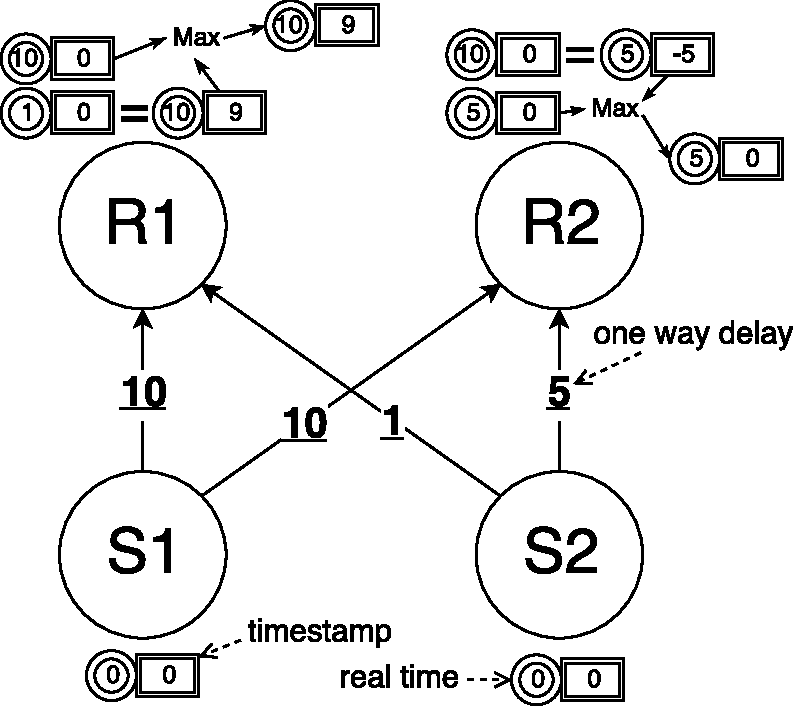
\includegraphics[width=.33\textwidth]{images/minimax_example_1.pdf}}
	%\hspace{0.08\textwidth}
	\subfloat[Backward aggregation (min) and RTT compensation.\label{fig:minimax_min}]
	{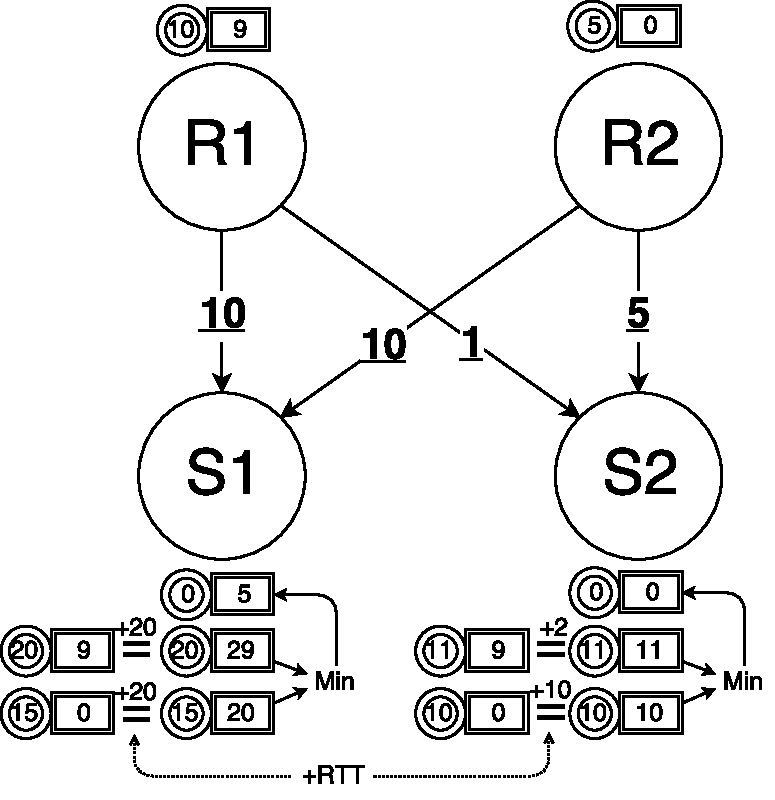
\includegraphics[width=.33\textwidth]{images/minimax_example_2.pdf}}
	%\hspace{0.08\textwidth}
	\subfloat[Reorder delay after synchronization.\label{fig:minimax_result}]
	{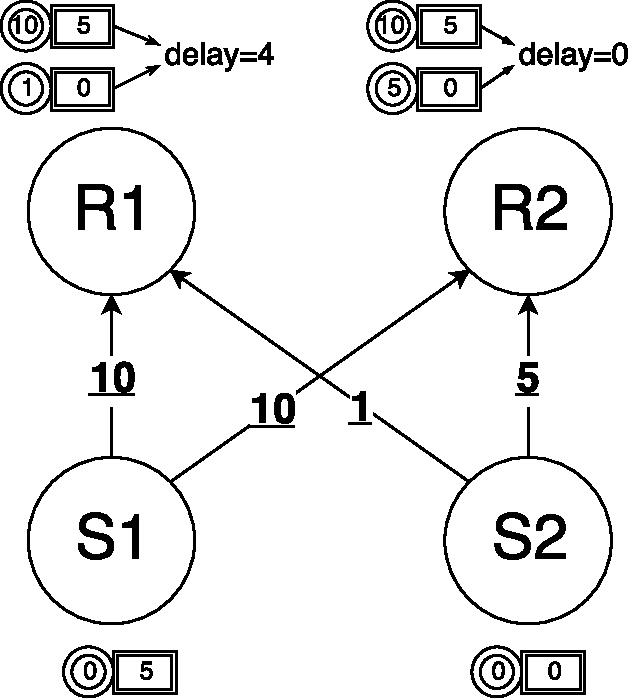
\includegraphics[width=.3\textwidth]{images/minimax_example_3.pdf}}

\caption{Illustration of minimax clock synchronization.}
\label{fig:minimax}
\vspace{-1.2em}
\end{figure*}

Fig.~\ref{fig:minimax} shows an example with two senders and two receivers.
In Fig.~\ref{fig:minimax_max}, each receiver chooses the maximum timestamp offset from physical clock and broadcasts the offset back to sender.
Initial reordering delays are 10 at $R_1$ and 5 at $R_2$.
In Fig.~\ref{fig:minimax_min}, each sender adds RTT to received offsets and synchronizes to the minimum offset.
Fig.~\ref{fig:minimax_result} shows that after minimax synchronization, reordering delays reduce to 4 at $R_1$ and 0 at $R_2$.
\fi


Without in-network computation, clock synchronization would require $O(N^2)$ messages.
Similar to hierarchical aggregation of barriers, we use network switches to aggregate \texttt{min} and \texttt{max} timestamps hierarchically.
% as shown in Algorithm~\ref{alg:minimax}.

\iffalse
The first property is necessary for correctness.
The second property ensures numerical stability, \textit{i.e.}, the increase speed of timestamps does not vanish or explode.
In addition, the second property enables us to obtain an unbiased estimate of the event timestamp after one round trip, by measuring RTT with a local physical clock.
The third property minimizes reordering delay by optimizing for simultaneous arrival of a message timestamp and its corresponding barrier timestamp.

To maintain the second property, we store event timestamps as \textit{offsets} relative to local physical clock on end hosts and switches.
When sending timestamps to the network, we add current clock time back to the offset.
This effectively uses physical clock to measure \textit{relative time} instead of absolute time, so the clock skew would not accumulate.
Physical clocks driven by crystal oscillators and CPU instruction counters are accurate enough to measure short intervals, because their relative error is less than $10^{-5}$~\cite{corbett2013spanner} and the granularity is at nanosecond level to ensure each packet has a unique timestamp.
It worth noting that Sec.~\ref{sec:ideal} stores a timestamp barrier as an \textit{absolute value} to represent a slacked bound, while this subsection stores event timestamps as \textit{relative offsets} to represent unbiased estimations.

For the third property, we determine new event timestamp on end hosts according to feedback information from the network.
The synchronized timestamp from the network may be smaller than the last assigned event timestamp $T_{last}$.
To prevent the event timestamps from decreasing, we track $T_{last}$ and let the new event timestamp to be the maximum of $T_{last} + 1$ and synchronized timestamp, as shown in Algorithm~\ref{alg:clock}.
This effectively ``stalls'' the event timestamp until the synchronized timestamp catches up with it.
\fi


\iffalse
To derive the timestamp feedback in the network, we need to estimate the delay from end-host senders to end-host receivers.
One-way delay is hard to measure, therefore we use round-trip time (RTT) instead.
Each end-host will add RTT to received feedback timestamp, just as illustrated in Figure~\ref{fig:minimax_min}.
When considering switches, one-hop RTT will be measured and compensated for feedback by each switch.

The challenge is that there are multiple senders and receivers, so we must aggregate timestamps from different hosts.
Let \texttt{FwdFunc} aggregate sender timestamps $T_i, i \in \mathcal{S}$ and \texttt{BackFunc} aggregate feedbacks from receivers $j \in \mathcal{R}$.
To simplify discussion, assume $d_{ij}$ is a fixed (but not measurable) one-way delay from sender $i$ to a receiver $j$, $r_{ji}$ is the fixed delay from receiver $j$ to sender $i$, and $RTT_{ij} = d_{ij} + r_{ji}$ is measurable.
The new event timestamp $T'_k$ on a sender $k \in \mathcal{S}$ is:

\begin{equation*}
\begin{aligned}
T'_k & = \texttt{BackFunc} \{ \texttt{FwdFunc} \{ T_i - d_{ij} \} - r_{jk} + RTT_{kj} \} \\
     & = \texttt{BackFunc} \{ \texttt{FwdFunc} \{ T_i - d_{ij} \} + d_{kj} \}
\end{aligned}
\end{equation*}

On one hand, because timestamps must grow monotonically, all clocks in the system should catch up with the clock with highest timestamp.
To this end, $T'_k$ needs to reflect the maximum of sender timestamps $T_i$.
Because $T_i, \forall i$ only appears in \texttt{FwdFunc}, \texttt{FwdFunc} needs to be $max$.

On the other hand, to ensure the second and fourth property of event timestamps, $\Sigma T_k, \forall k$ should converge.
Choosing \texttt{BackFunc} as $min$ and \texttt{FwdFunc} as $max$ guarantees that each timestamp converge after one RTT for any initial assignment of $T_k$, \textit{i.e.}, $\forall k, T'_k = T''_k$.
This self-stabilization property is proved in Appendix \ref{appx:minimax}.

Figure~\ref{fig:minimax} is a simple example of minimax synchronization.
The network consists of only two senders and two receivers.
In Figure~\ref{fig:minimax_max}, both senders assign timestamp to $0$ at the very beginning (equivalent to physical clock synchronized).
Based on linear time assumption, both receivers choose the maximum timestamp as feedback.
In Figure~\ref{fig:minimax_min}, both senders add RTT to feedback and synchronize to the minimum feedback timestamp.
Figure~\ref{fig:minimax_result} shows that compared to the original timestamp assignment, reorder delay declines after minimax synchronization.

Finally, to reduce the message complexity of clock synchronization, we use network switches to aggregate the $min$ and $max$ timestamps hierarchically.
%as shown in Algorithm~\ref{alg:minimax}.
\fi

\iffalse

\setlength{\textfloatsep}{0em}
\begin{algorithm}[t]
 \DontPrintSemicolon
 \textbf{States:} Max timestamp per input link, $max_i, i \in \mathcal{I}$\;
 	\qquad Min timestamp per output link, $min_o, o \in \mathcal{O}$\;
    \qquad RTT estimation per output link, $RTT_o, o \in \mathcal{O}$\;
    \qquad Received RTT probe request, $rttreq_i, i \in \mathcal{I}$\;
 	\qquad Local physical clock, fetched via $time()$\;
 \textbf{Event processing:}\\
 \If{send beacon packet to port $P$}{
    piggyback the following with the beacon packet:\\
 	max timestamp $T_{max}$:\\
    \quad $T_{max} = \max \{ max_i | i \in \mathcal{I} \wedge i \rightarrow P \} + time()$\;
    min timestamp $T_{min}$:\\
    \eIf{$\exists o, o \in \mathcal{O} \wedge P \rightarrow o$} {
        $T_{min} = \min \{ min_o | o \in \mathcal{O} \wedge P \rightarrow o \} + time()$\;
    }{
    	$T_{min} = T_{max}$\;
    }
    RTT probe request $rtt_{req}$:\\
    \quad $rtt_{req} = time()$\;
    RTT probe response $rtt_{ack}$:\\
    \quad $rtt_{ack} = time() - rttreq_P$\;
 }
 \ElseIf{received beacon packet from port $P$}{
    extract $T_{max}, T_{min}, rtt_{req}, rtt_{ack}$ from beacon\;
    $RTT_P \leftarrow \alpha \cdot (time() - rtt_{ack}) + (1 - \alpha) \cdot RTT_P$\;
 	$max_P \leftarrow T_{max} - time()$\;
    $min_P \leftarrow T_{min} + RTT_P - time()$\;
    $rttreq_P \leftarrow time() - rtt_{req}$\;
 }
 \caption{Minimax clock synchronization on each network switch and end host (treated as a single-port switch).}
 \label{alg:minimax}
\end{algorithm}

\fi

%One may ask why we use physical clock instead of Lamport clock (cite) or vector clock (cite) to measure intervals. A clock measures an interval by counting repetitive events. A good clock source should generate a roughly same number of repetitive events when our measurement object is stable, as well have a granularity finer than the intervals to measure.
%If we use packet counter as clock source, the RTT measurement will vary with network throughput. If we use received timestamps as clock source, it is unable to measure a tiny interval if no packet is received during the interval. Physical clocks driven by crystal oscillators and CPU instruction counters are accurate enough to measure short intervals, because their relative error is less than $10^{-5}$ (cite) and the granularity is as fine as a nanosecond.



\section{\sys in Unreliable Networks}
\label{sec:design-unreliable}

Previous section describes \sys in reliable networks. In this section, we discuss how to maintain the ordering and atomicity of message delivery in the presence of packet losses and node failures.

\subsection{Packet Loss Detection and Recovery}
\label{sec:lossy}
%In addition, some devices or network links may have congestion or bugs that lead to higher packet loss possibility~\cite{guo2015pingmesh}.

\parab{Problem.}In data centers, the packet corruption rate is around $10^{-5}$ \texttildelow $10^{-7}$~\cite{zhuo2017understanding}. In addition, packets get dropped due to congestion and device bugs~\cite{guo2015pingmesh}. Due to packet losses, the barrier timestamp is inefficient for message delivery because messages might get dropped and retransmitted. If messages are immediately delivered when their timestamps are below the barrier, a retransmitted message with lower timestamp may get delivered out of order. 

To address this problem, a traditional solution is two-phase commit (2PC). In 2PC, each receiver responds an ACK to a data message, then the sender multicasts a commit message after receiving all ACKs, receivers then deliver the data when receiving the commit message. This approach requires three one-way delays when no packet loss happens.

\parab{Solution.}We aim to deliver messages with an one-way delay when no packet loss happpens, and fall back to the 2PC-like protocol when any packet loss happens. To achieve this, \sys leverages NICs and switches to detect packet losses. Hosts locate and retransmit lost packets via TCP-like loss recovery.

%\sys detects packet losses on last-hop links and queues using packet loss counter in NICs and switches. Given the limited switch buffer resource, we rely on end hosts to locate and retransmit lost packets via TCP-like loss recovery.
%Since retransmitted packets may violate the barrier property, we add a special mark to them.

%Due to packet loss, the barrier timestamp is no longer sufficient for message delivery because message might get dropped and retransmitted. If messages are immediately delivered when their timestamp is below the barrier, a retransmitted message with lower timestamp may get delivered out of order. Our aim is to deliver messages in one-way network delay when no packet loss is encountered, and fall back to a protocol similar to two-phase commit (2PC) with three one-way delays when loss occurs.

In \sys, we rename the original barrier to \textit{loss-free barrier} and add a \textit{delivery barrier} field and a \textit{loss encountered} flag to each packet.
Delivery barrier carries accumulative delivery timestamp from the sender, which means that all messages sent by the sender and below delivery barrier have been delivered. Figure~\ref{fig:ack-barrier} shows an example of delivery barrier. When loss encountered flag is off, a receiver can deliver messages according to the loss-free barrier. Otherwise, it delivers based on delivery barrier.

When packet loss is encountered, we use a protocol similar to 2PC to update the delivery barrier. 
In \sys, the receiver replies ACKs to the sender when it receives a message.
Then the message is buffered as a prepared message, not delivered.
Unlike regular 2PC, \sys can only deliver a message after delivering all messages with lower timestamps.
Instead of multicasting commit messages, the sender sends messages with updated delivery barrier.
\sys hierarchically aggregates updated delivery barriers in network so that receivers know the timestamp lower bound of all delivered (and prepared) messages and can deliver the prepared messages accordingly.

When delivery barrier catches up with loss-free barrier recorded at last packet loss, the switch clears loss encountered flag, thus enables receivers to deliver messages without waiting for an additional RTT.

At this time, messages below delivery barrier are received and messages above that are not lost before passing through this switch. This is shown in Algorithm~\ref{alg:loss-detection}, 




\setlength{\textfloatsep}{1em}
\begin{algorithm}[t]
 \DontPrintSemicolon
 \textbf{States:} Loss-free barrier $UB_i, i \in \mathcal{I}$\;
 	\qquad Delivery barrier $CB_i, i \in \mathcal{I}$\;
    \qquad Received loss encountered flag $RLE_i, i \in \mathcal{I}$\;
 	\qquad Last-hop loss encountered flag $LE_i, i \in \mathcal{I}$\;
    \qquad Loss-free barrier at last loss $LB_i, i \in \mathcal{I}$\;
    \qquad Last loss counter $LC_i, i \in \mathcal{I}$\;
    \qquad Current loss counter, fetched via $C(i), i \in \mathcal{I}$\;
 \textbf{Event processing:}\\
 \If{\textnormal{Receive beacon from input link $i$}}{
 	$RLE_i \leftarrow$ loss encounter flag in the packet\;
    $UB_i \leftarrow$ loss-free barrier in the packet\;
    $CB_i \leftarrow$ delivery barrier in the packet\;
    \If{$LC_i \neq C(i)$}{
    	$LE_i \leftarrow \textnormal{True}$\;
        $LB_i \leftarrow UB_i$\;
        $LC_i \leftarrow C(i)$\;
    }
	\ElseIf{$CB_i \geq LB_i$}{
    	$LE_i \leftarrow \textnormal{False}$\;
    }
 }
 \ElseIf{\textnormal{Send beacon to output link $o$}}{
    Loss-free barrier $\leftarrow \min \{ UB_i | i \in \mathcal{I} \wedge i \rightarrow o \}$\;
	Delivery barrier $\leftarrow \min \{ CB_i | i \in \mathcal{I} \wedge i \rightarrow o \}$\;
    Loss encountered flag $\leftarrow \exists i \in \mathcal{I} \wedge (i \rightarrow o) \wedge (LE_i \vee RLE_i)$\;
 }
 \caption{Hop-by-hop loss detection in network switches.}
 \label{alg:loss-detection}
\end{algorithm}

%To detect packet loss in the network, we leverage per-port packet loss counter in commodity NICs and switches.
%If packet loss counter of an input link changes, we know that a packet is lost during current interval and set the \textit{loss encountered} flag of the input link.
%As a justification, our actual measurements find that the number of end-to-end packet losses agree with the packet drop counters in our test environment.


\begin{figure}[t]
\centering
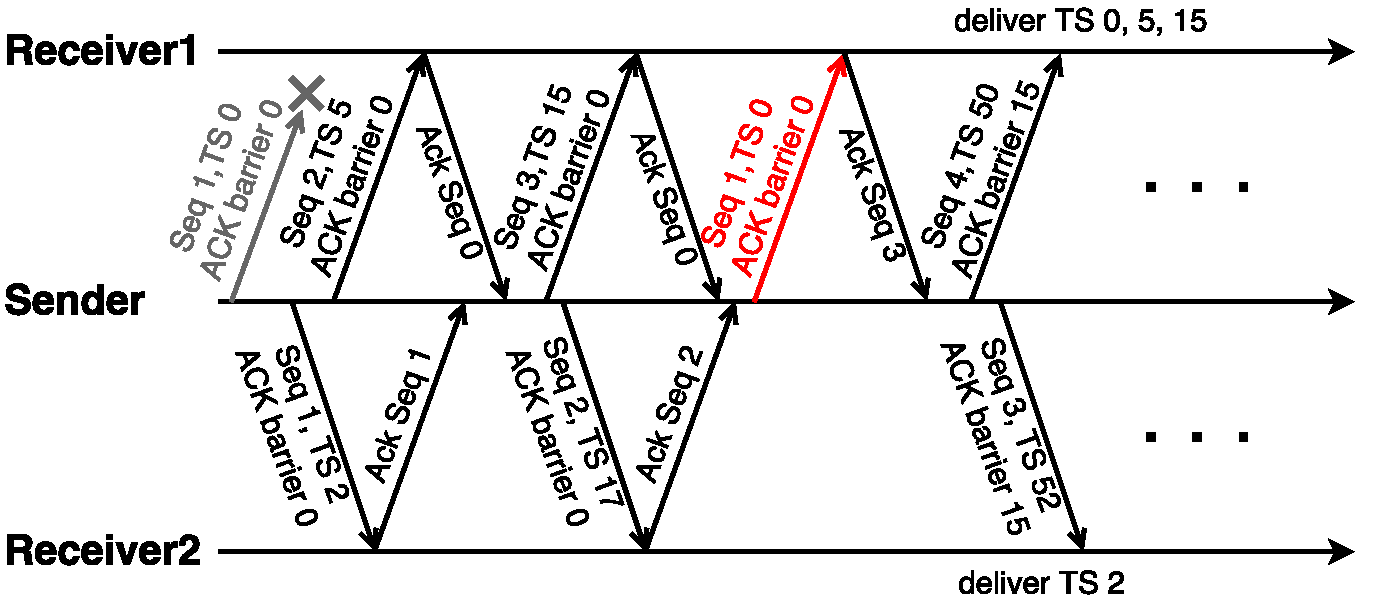
\includegraphics[width=0.45\textwidth]{images/loss_detection.pdf}
\caption{Loss recovery and delivery barriers.}
\label{fig:ack-barrier}
\vspace{-0.4em}
\end{figure}



%Similar to TCP, packets have sequence numbers independent of timestamps.
%The receiver responds ACK to the sender via non-timestamped packets.
%For each connection, the sender maintains a \textit{minimum unacknowledged timestamp}, detect packet loss via duplicate ACKs or timeout, then retransmit the lost packets with the same timestamp (Figure~\ref{fig:ack-barrier}).
%Each sender maintains an unacknowledged timestamp barrier (\textit{ACK barrier}), which is the minimum of minimum unacknowledged timestamps among all connections. Messages with timestamps below the ACK barrier are guaranteed to be received by all recipients.

\subsection{Fault Tolerance and Incremental Deployment}
\label{sec:failure}

Previous section retransmits lost packets with end hosts.
When a host, switch or network link fails, barrier timestamps and message delivery stall.
We detect failures using beacon timeout and remove failed nodes to resume progress of rest of the system.
Because failures and packet loss can be detected, achieving atomicity is much easier than consensus in general distributed systems.

First, we deal with host failure.
When a host fails, the nearby switch will detect it via beacon timeout and broadcast the failure in beacon packets.
A receiver discards messages from the failed node in reordering buffer.
To ensure message scattering atomicity, a sender checks undelivered messages and send \textit{recall} messages to other receivers.
Upon receiving \textit{recall}, the receiver discards the message in reordering buffer and responds ACK.
The sender then discards the undelivered message when all healthy receivers have recalled.
We admit that \sys shares the same limitation with standard two-phase commit.
If a receiver fails after delivery barrier has been sent, \sys cannot recall delivered messages from other receivers.

When a host recovers from failure, it needs to join \sys system as a new host.
Recovering lost messages during failure requires persistence or replication, which incurs high cost. So the best choice is to let applications determine, rather than \sys transport.

Next, we deal with failure of network switches or links.
If a failure does not block communication between any pair of hosts, it only causes a brief interval of packet losses.
Otherwise, the sender would timeout in retransmission and \textit{recall} messages from other receivers.
If a failure disconnects an end host from the network (\textit{e.g.} ToR switch failure), nearby switches would broadcast the host failure.
%\RED{Q1:should every switch records which host may pass through which input link? so that the switch is able to broadcast (potential) host failure. It seems really difficult. Q2:What if switches hold different opinions about whether a host fails. Is it possible?}
In the extreme case of network partition, all cross-partition scatterings will fail and scatterings within a partition still proceed with total order.

%Switches and end hosts detect network link or neighbor node failure when no beacons are received within a timeout interval.
%Upon detection of failure, it will install a firewall rule to block data packets from the corresponding port and excludes the port from barrier aggregation and clock synchronization.
%As an effect, the barriers are temporarily stalled during the timeout interval, and proceed to increase after the failure port is excluded.
%In terms of CAP theorem~\cite{brewer2000towards}, we choose availability and partition tolerance over consistency between the partitions.
%When the link or neighbor node recovers, it needs to rejoin the \sys system like a newcomer.

%When an end host or switch needs to join a \sys system, it first initializes a \sys system by itself (all the timestamps are initialized arbitrarily). Therefore, the joining process is reduced to connecting two existing \sys systems with a new network link.


Failure recovery and incremental deployment requires new hosts, switches and links to join a \sys system efficiently.
All these cases can be reduced to adding a link $L$ between two nodes.
Initially, the nodes block all data packets on $L$ and only allow beacon packets carrying barriers and clock synchronizations.
A node adds $L$ to its input links list only when the barrier from $L$ isn't smaller than the minimum barrier of existing input links.

With minimax clock synchronization, the entire network synchronize clocks in one RTT, since then the barriers would meet the condition.
Consequently, only one RTT is required for failure recovery and adding new nodes.
Since adding a host has low latency overhead, when a host stops using \sys, it can notify the switch its exit and stop sending beacons, but it must rejoin before sending messages again.

\iffalse
\subsection{Inter-DC Topology}
\label{sec:inter-dc}


\begin{figure}[t]
\centering
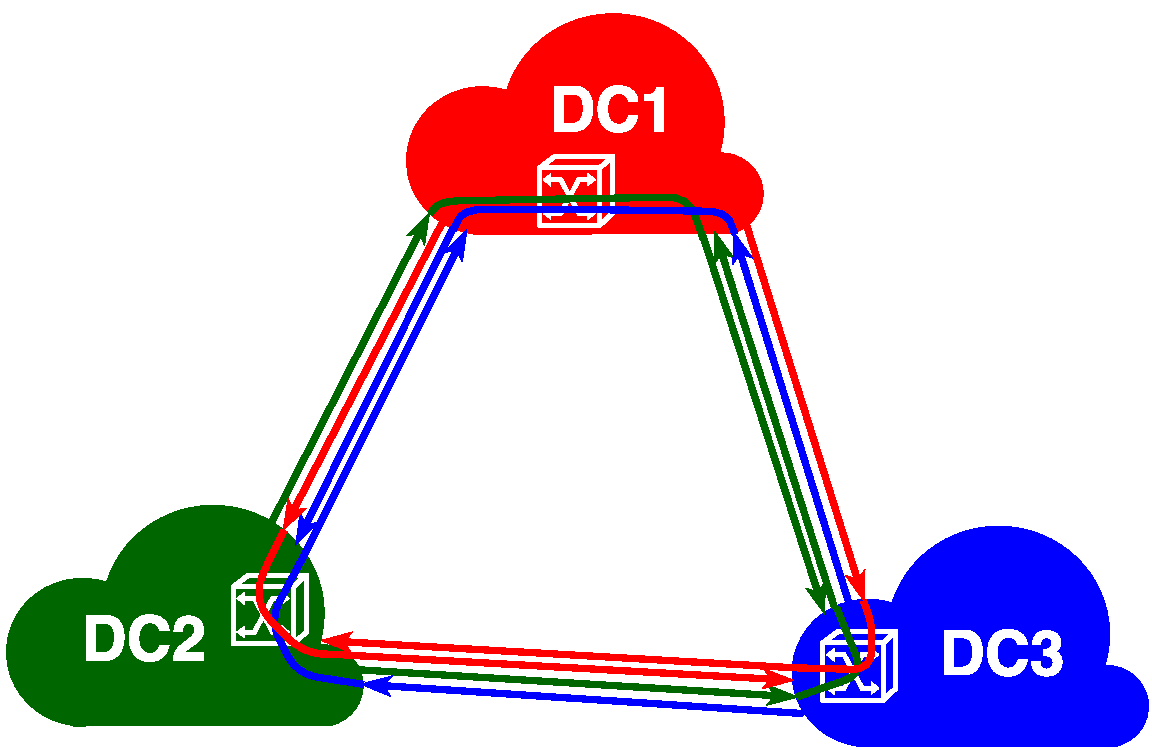
\includegraphics[width=0.48\textwidth]{images/inter-DC.pdf}
\caption{
	Partition an inter-DC network to multiple shards.
	Each color indicates a shard composed of one DC and the virtual routing paths originating from the DC.
}
\label{fig:inter-dc}
\end{figure}



Intra-datacenter (intra-DC) routing paths are typically loop-free (Sec.~\ref{sec:dcn}), leading to efficient hierarchical aggregation.
However, inter-DC routing paths are typically not loop-free.
Fortunately, there is typically no ``hairpin'' traffic in inter-DC routing tables: packets passing through DC $A$ will never pass through some other DC $B$ and come back to $A$.

We partition the inter-DC network to $N$ logical shards, where $N$ is the number of DCs.
Each shard is composed of one unique DC and all inter-DC traffic originating from the DC.
Therefore, each inter-DC link is logically split to $N$ logical links, each carrying traffic originating from one DC.
The partitioning can be implemented by tagging each packet with an origin DC ID.
In this way, each switch in inter-DC WAN is logically split into $N$ switches, and at most $N$ beacon messages per inter-DC link are needed in each beacon interval.
Because the routes in each shard originate from a same DC, they form a DAG and are loop-free by our definition.\RED{(confused, loop-free logical shard leads to what?)}
Note that loop-free only affects liveness and is not required by correctness, therefore temporary routing loops will only stall message delivery until the loop disappears.

Typically, transit traffic of a DC only goes through border switches, analogous to ``international zones'' in an airport.
If this is the case, we can handle intra-DC traffic as if no other DCs are present.
For an incoming packet from another DC, the border switch removes the origin DC tag; for an outgoing packet, the border switch adds the origin DC tag.
\fi
